\paragraph{IUE03.1 Registrar rutina} \hspace{1cm}\\ 
\label{pant:IUE03.1}

\textbf{\textcolor[rgb]{0, 0, 0.545098}{Objetivo}}\\
Esta pantalla permite al Entrenador registrar una nueva rutina de entrenamiento, solicitando al Entrenador la información necesaria para registrarla en la herramienta.\\

\textbf{\textcolor[rgb]{0, 0, 0.545098}{Diseño}}\\
La figura \ref{fig:IUE03.1} muestra al Entrenador un grupo de elementos, en los cuales se enlistan los Ejercicios de calentamiento y Movimientos de técnica disponibles para registrar en un nueva rutina de entrenamiento, así como para registrar las repeticiones de cada movimiento y los identificadores de la rutina.\\

En la parte inferior se encuentran los botones de Guardar y Cancelar, los cuales corresponden a registrar una rutina o bien, cancelar el registro.

\begin{figure}[H]
	\centering
		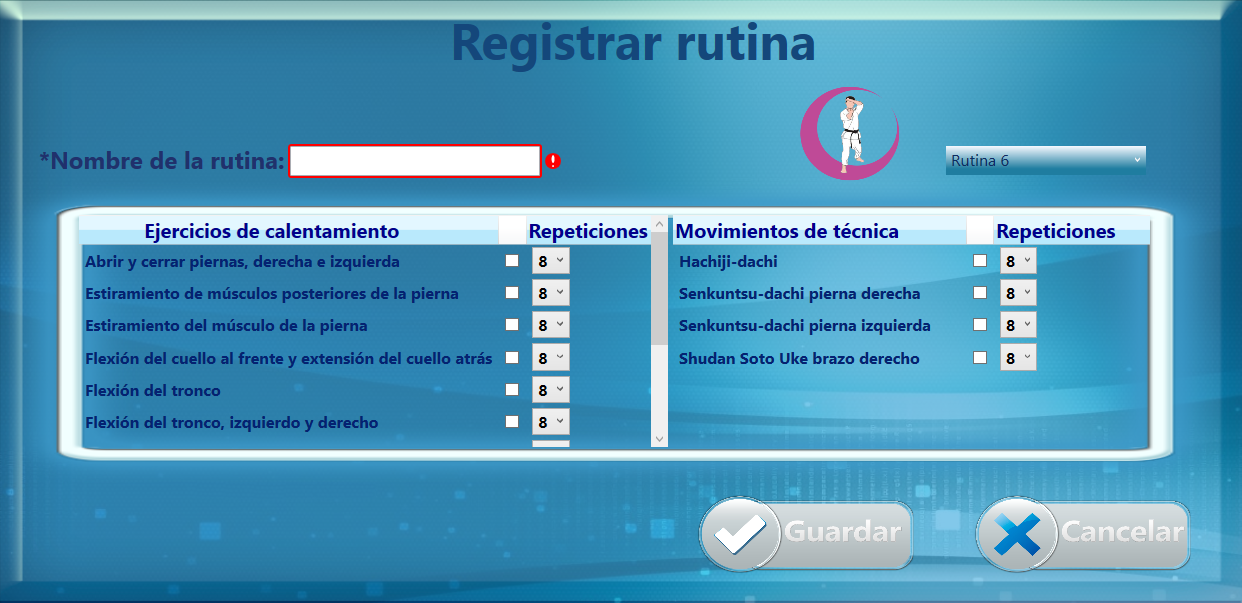
\includegraphics[scale=0.5]{./Figuras/Pantallas/IUE03_1Registrar_rutina}
	\caption{IUE03.1 Registrar rutina}
	\label{fig:IUE03.1}
\end{figure}

\textbf{\textcolor[rgb]{0, 0, 0.545098}{Entradas}}\\
En esta pantalla el Entrenador deberá capturar la siguiente información:

\begin{itemize}
	\item El Nombre de la nueva rutina a registrar.
\end{itemize}
\vspace{1em}

\textbf{\textcolor[rgb]{0, 0, 0.545098}{Controles}}
\begin{itemize}
	\item \textbf{\textcolor[rgb]{0, 0, 0.545098}{Calentamiento:}} Permite seleccionar al Entrenador ejercicios de calentamiento que desea registrar en la nueva rutina de entrenamiento. 
	\item \textbf{\textcolor[rgb]{0, 0, 0.545098}{Técnica:}} Permite seleccionar al Entrenador movimientos de técnica que desea registrar en la nueva rutina de entrenamiento.
	\item \textbf{\textcolor[rgb]{0, 0, 0.545098}{Repeticiones:}} Permite seleccionar al Entrenador el número de repeticiones disponibles para cada movimiento o ejercicio seleccionado.
	\item \textbf{\textcolor[rgb]{0, 0, 0.545098}{Seleccionar imagen descriptiva:}} Permite seleccionar al Entrenador una imagen alusiva a la rutina de entrenamiento que desea registrar.
\end{itemize}
\vspace{1em}

\textbf{\textcolor[rgb]{0, 0, 0.545098}{Comandos}}
\begin{itemize}
	\item \textbf{\textcolor[rgb]{0, 0, 0.545098}{Guardar:}} Permite al Entrenador registrar una nueva rutina de entrenamiento cuando la información ingresada en los campos obligatorios sea correcta.
	\item \textbf{\textcolor[rgb]{0, 0, 0.545098}{Cancelar:}} Descarta la información registrada y muestra la pantalla \nameref{pant:IUE03}.
\end{itemize}
\vspace{1em}

\textbf{\textcolor[rgb]{0, 0, 0.545098}{Mensajes}}\\

\textbf{\nameref{msj:MSG01}}: Se muestra en la pantalla \nameref{pant:IUE03.1} cuando el Entrenador haya registrado a la rutina en la herramienta de manera exitosa.\\

\textbf{\nameref{msj:MSG02}}: Se muestra en la pantalla \nameref{pant:IUE03} cuando no existan elementos registrados en los catálogos correspondientes.\\

\textbf{\nameref{msj:MSG12}}: Se muestra en la pantalla \nameref{pant:IUE03.1} cuando el Entrenador no haya ingresado datos a los campos obligatorios.\\

\textbf{\nameref{msj:MSG13}}: Se muestra en pantalla el  cuando el Entrenador haya ingresado datos con formato incorrecto en un campo.\\

\textbf{\nameref{msj:MSG16}}: Se muestra en pantalla cuando el Entrenador no haya seleccionado al menos 3 ejercicios de calentamiento o cuando haya seleccionado más de 5 ejercicios y cuando el Entrenador no haya seleccionado al menos 2 movimientos de técnica o cuando haya seleccionado más de 4 movimientos.\\

\textbf{\nameref{msj:MSG20}}: Se muestra en pantalla el  cuando el Entrenador haya excedido el número de registros de rutinas permitidos.\\

\clearpage